\documentclass[12pt]{article}
\everymath{\displaystyle}
\usepackage{unicode-math}
\usepackage{pgfplots}
\pgfplotsset{compat=1.18}
\usepackage{amsmath}


\usepackage[margin=1in]{geometry}
\usepackage{tcolorbox}
\usepackage{graphicx}
\usepackage{tikz}
\usepackage{amssymb}
\usepackage{enumitem}
\usepackage{titlesec}
\usepackage{fancyhdr}
\usepackage{pifont}
\usepackage{xcolor}
\newcounter{questionnum}
\setcounter{questionnum}{0}
\usepackage{eso-pic} % for page background

% --------- 主题颜色设置 ---------
\definecolor{novelblue}{RGB}{70,60,150}
\definecolor{headerbg}{RGB}{240,240,255}

\pagestyle{fancy}
\fancyhf{}
\renewcommand{\headrulewidth}{0.4pt}
\renewcommand{\headrule}{\hbox to\headwidth{\color{novelblue}\leaders\hrule height 0.4pt\hfill}}

% --------- 页眉背景色条 ---------
\newcommand{\headbackground}{
  \AddToShipoutPictureBG*{
    \begin{tikzpicture}[remember picture, overlay]
      \fill[blue!5!purple!10] (current page.north west) rectangle ([yshift=-60pt]current page.north east);
    \end{tikzpicture}
  }
}

% --------- 页眉设置 ---------
\pagestyle{fancy}
\fancyhf{}
\renewcommand{\headrulewidth}{0pt}
\fancyhead[L]{\color{novelblue}\textbf{\textbf{Novel Prep} }}
\fancyhead[C]{\color{novelblue}\textbf {SAT Preparation}}
\fancyhead[R]{\color{novelblue}\textbf{Jack Zeng}}


\newtcolorbox{SATCard}[1][]{%
  enhanced,
  colback=white,
  colframe=novelblue,
  coltitle=white,
  boxrule=0.6pt,
  arc=4pt,
  boxsep=5pt,
  left=8pt, right=8pt, top=10pt, bottom=10pt,
  sharp corners=south,
  drop shadow south east,
  #1
}

% --------- 顶部 Mark for Review 栏 ---------
\newcommand{\markforreview}{
  \stepcounter{questionnum} % 自动递增题号
  \begin{tikzpicture}[scale=1.1]
    % 黑色题号
    \fill[black] (0,0) rectangle (0.8,0.6);
    \node[white, font=\bfseries\large] at (0.4,0.3) {\thequestionnum};

    % 灰底主栏
    \fill[gray!10] (0.8,0) rectangle (14.5,0.6);

    % Mark for Review
    \node[anchor=west, font=\small] at (1.2,0.3) {\ding{72} \hspace{2pt}Mark for Review};

    % ABC 按钮区域
    \draw[thick, rounded corners=3pt] (13.5,0.12) rectangle (14.5,0.48);
    \node[font=\bfseries\normalsize] at (14.0,0.3) {ABC};
  \end{tikzpicture}


  \newcommand{\choiceboxcircled}[2]{%
  \begin{tcolorbox}[
    colback=white,
    colframe=black,
    boxrule=0.5pt,
    rounded corners=6pt,
    left=6pt, right=6pt, top=6pt, bottom=6pt,
    width=\linewidth
  ]
    \textbf{\large\textcircled{\textbf{#1}}} \ #2
  \end{tcolorbox}
}
}

% --------- 选项框样式 ---------
\newcommand{\choicebox}[2]{%
  \begin{tcolorbox}[
    colback=white, 
    colframe=novelblue,
    boxrule=0.5pt, 
    rounded corners=4pt, 
    left=6pt, right=6pt, top=6pt, bottom=6pt,
    width=\linewidth
  ]
  \textbf{#1.} \ #2
  \end{tcolorbox}
}


\begin{document}
\section*{SAT Math Test 1}

\noindent\markforreview
\vspace{1em}

In the given expression, \(a\) and \(c\) are positive constants. If \(px + q\) is a factor of the expression,
\[
ax^2 + 176x + c = (px + q)(rx + s),
\]
where \(p\) and \(q\) are positive constants, what is the greatest possible value of \(ac\)?

\vspace{2em}

\noindent\markforreview
\vspace{1em}

In the given expression,
\[
34z^{18} + b z^9 + 30,
\]
\(b\) is a positive integer. If \(qz^9 + r\) is a factor of the expression, where \(q\) and \(r\) are positive integers, what is the greatest possible value of \(b\)?

\vspace{2em}

\noindent\markforreview
\vspace{1em}

The expression
\[
6x^4 + 17x^2 + 7
\]
can be rewritten as \((3x^2 + a)(2x^2 + b)\), where \(a\) and \(b\) are positive integers, or as \((3x^2 + c)(2x^2 + d)\), where \(c\) and \(d\) are positive non-integers.

What is the value of \(a + c\)?

\vspace{2em}

\noindent\markforreview
\vspace{1em}

The given quadratic function
\[
54x^4 + 219x^2 + 105
\]
has factors in the form \((k)(ax^2 + b)(cx^2 + d)\). If \(a, b, c, d, k\) are integers, what is the smallest possible value of \(ab\)?

\newpage

\noindent\markforreview
\vspace{1em}

The equation of a parabola is written in the form
\[
y = ax^2 + bx + c,
\]
where \(a, b, c\) are constants. When graphed in the \(xy\)-plane, the parabola has vertex \((-1, 4)\) and does not intersect the \(x\)-axis. Which of the following could be the value of \(a - b - c\)?

\choicebox{A}{2}
\choicebox{B}{4}
\choicebox{C}{-1}
\choicebox{D}{-6}

\vspace{2em}

\noindent\markforreview
\vspace{1em}

A quadratic function with vertex \((1, 32)\) can be written as
\[
 -ax^2 + bx + c \quad (a, b, c \text{ are all positive integers}).
\]
What is the maximum value of \(b\)?

\vspace{2em}

\noindent\markforreview
\vspace{1em}

An object’s speed is increasing at a rate of \(7.7\ \text{meters per second squared}\). What is this rate in \textbf{miles per minute squared}, rounded to the nearest tenth? (Use \(1\ \text{mile} = 1609\ \text{meters}\).)

\vspace{0.75em}

\choicebox{A}{0.3}
\choicebox{B}{17.2}
\choicebox{C}{206.5}
\choicebox{D}{209}

\vspace{2em}

\noindent\markforreview
\vspace{1em}

The function \(f\) is defined by
\[
f(x) = ab^{x/n},
\]
where \(a, b, n\) are constants, and \(b, n\) are integers. If \(f(2) = 6\) and \(f(4) = 150\), what is the value of \(f(5)\)?

\vspace{3em}

\noindent\markforreview
\vspace{1em}

The graph of \(y = f(x)\) in the \(xy\)-plane has a vertex at \((4, -7)\), contains the point \((3, -9)\), and has a \(y\)-intercept at \((0, a)\). The graph of \(y = 6 \cdot f(x)\) has a \(y\)-intercept at \((0, b)\). What is the positive difference between \(a\) and \(b\)?

\vspace{2em}

\noindent\markforreview
\vspace{1em}

The function \(f\) is defined by
\[
f(x) = ax^2 + bx + c,
\]
where \(a, b, c\) are constants. The graph of \(y = f(x)\) passes through the points \((9, 0)\) and \((-2, 0)\). If \(a\) is an integer greater than 1, which of the following could be the value of \(a + b\)?

\vspace{0.75em}

\choicebox{A}{8}
\choicebox{B}{7}
\choicebox{C}{-6}
\choicebox{D}{-12}


\vspace{2em}
\newpage
\noindent\markforreview
\vspace{1em}

Which of the following expressions has a factor of \(x + 2b\), where \(b\) is a positive integer constant?



\choicebox{A} {3x^2 + 7x + 14b}
\choicebox{B}{3x^2 + 22x + 14b}
\choicebox{C}{3x^2 + 30x + 14b} 
\choicebox{D}{3x^2 + 37x + 14b} 


\noindent\markforreview
\begin{center}
    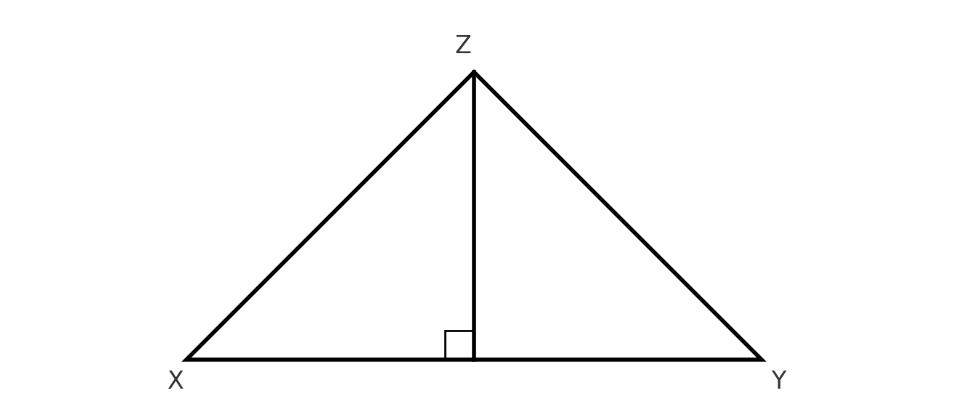
\includegraphics[width=0.5\linewidth]{f1.png}
\end{center}


In the figure shown, the measure of angle \(Y\) is \(38^\circ\). The length of \(XY\) is 12 meters, and the length of \(YZ\) is 5 meters. What is the area, in square meters, of triangle \(XYZ\)?

\vspace{0.75em}

\choicebox{A}{30}
\choicebox{B}{60}
\choicebox{C}{30 \sin 38^\circ}
\choicebox{D}{60 \sin 38^\circ}

\newpage

\noindent\markforreview
\vspace{1em}

A research manager selected two random samples to estimate the average lifespan of a certain type of light bulb (in hours). Based on the first sample, the research manager estimated that the average lifespan of this type of light bulb is 800 hours, with a margin of error of 20 hours.

Based on the second sample, the research manager estimated that the average lifespan of this type of light bulb is 810 hours, with a margin of error of 35 hours.

Assuming the margins of error were calculated in the same way, which of the following best explains why the first sample obtained a smaller margin of error than the second sample?

\vspace{0.75em}

\choicebox{A}{The first sample contained fewer light bulbs than the second sample.}
\choicebox{B}{The first sample contained more light bulbs than the second sample.}
\choicebox{C}{The first sample had a shorter average lifespan than the second sample.}
\choicebox{D}{The first sample had a longer average lifespan than the second sample.}

\vspace{2em}

\noindent\markforreview
\vspace{1em}

The function \(p(x)\) is defined by:
\[
p(x) = a((x - 3)^2 + b)((x - 3)^2 - c),
\]
where \(a, b,\) and \(c\) are constants. The graph of \(y = p(x)\) passes through the points \((1, 25)\) and \((-1, 52)\).

What is the value of \(p(5) + p(7)\)?

\vspace{0.75em}

\choicebox{A}{25}
\choicebox{B}{27}
\choicebox{C}{52}
\choicebox{D}{77}

\vspace{2em}

\noindent\markforreview
\vspace{1em}

In the given function, \(b\) is a positive constant. For every increase in the value of \(x\) by 1, the value of \(f(x)\) increases by \(c\%\), where \(0 < c < 100\).

Which expression gives the value of \(c\) in terms of \(b\)?
\[
f(x) = 66(b)^x

\]

\vspace{0.75em}

\choicebox{A}{ 1+ $\frac{b}{100}$$}
\choicebox{B}{b + 100}
\choicebox{C}{100(b + 1)}
\choicebox{D}{100(b - 1)}

\vspace{2em}

\noindent\markforreview
\vspace{1em}

On average, a certain tree grows 87 centimeters every \(m\) months. At this rate, which expression represents the number of centimeters, on average, the tree grows every \(k\) years?

\vspace{0.75em}

\choicebox{A}{\dfrac{29m}{4k}}
\choicebox{B}{\dfrac{29k}{4m}}
\choicebox{C}{\dfrac{1044m}{k}}
\choicebox{D}{\dfrac{1044k}{m}}

\vspace{2em}

\noindent\markforreview
\begin{center}
    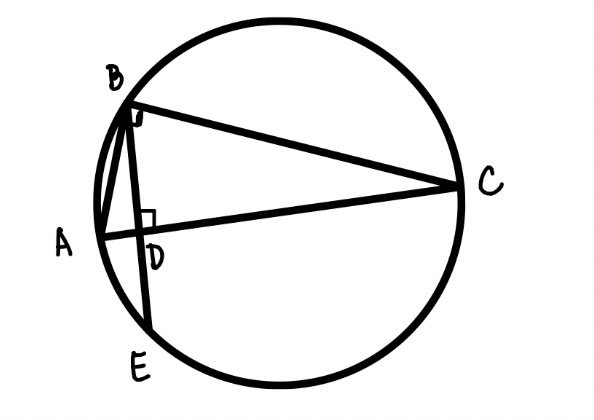
\includegraphics[width=0.5\linewidth]{f2.jpg}
\end{center}


In the figure shown, points \(A, B, C,\) and \(E\) lie on the circle, and \(AB < BC\). Segment \(AC\) is perpendicular to segment \(BE\) at point \(D\), and \(BD = \sqrt{346}\). The diameter of the circle is 175. If \(\dfrac{CD}{AD} = r\), what is the value of \(r\)?

\vspace{2em}

\noindent\markforreview
\vspace{1em}

In the given equation, \(a\) and \(k\) are constants, where \(k > 5a\). The sum of the solutions to the equation is \(3k + 32\). What is the value of \(a\)?
\[
(x - k)^2 = (k - 5a)(x - k)
\]

\vspace{0.75em}

\choicebox{A}{-\dfrac{32}{5}}
\choicebox{B}{\dfrac{32}{5}}
\choicebox{C}{-\dfrac{5}{32}}
\choicebox{D}{\dfrac{5}{32}}

\vspace{2em}
\newpage
\noindent\markforreview
\vspace{1em}

The equation \(N(m) = 63(Q)^{m/6}\) gives the predicted population \(N(m)\), in thousands, of a certain bacteria colony \(m\) minutes after the initial measurement, where \(Q\) is a constant greater than 1. The predicted population increases by \(p\%\) every 180 seconds.

What is the value of \(p\) in terms of \(Q\)?

\vspace{0.75em}

\choicebox{A}{100(Q^{30} - 1)}
\choicebox{B}{100(Q^{\frac{1}{2}} - 1)}
\choicebox{C}{100(Q^{30} + 1)}
\choicebox{D}{100(Q^{1.5} + 1)}

\vspace{2em}

\noindent\markforreview
\vspace{1em}

In the given equation, \(m\) and \(n\) are constants. The sum and product of the solutions of the equation are 8 and \(\dfrac{7}{2}\), respectively.

What is the value of \(\dfrac{m}{n}\)?
\[
(x - m)^2 = (m + 2n)(2x - n)
\]

\vspace{0.75em}

\choicebox{A}{-\dfrac{1}{3}}
\choicebox{B}{\dfrac{1}{3}}
\choicebox{C}{-3}
\choicebox{D}{3}

\newpage

\noindent\markforreview
\vspace{1em}

One gallon of stain will cover 170 square feet of a surface. A yard has a total fence area of $w$ square feet.  
Which equation represents the total amount of stain $S$, in gallons, needed to stain the fence in this yard twice?
\vspace{0.75em}

\choicebox{A}{$S = \dfrac{w}{170}$}  
\choicebox{B}{$S = 170w$}  
\choicebox{C}{$S = 340w$}  
\choicebox{D}{$S = \dfrac{w}{85}$}


\vspace{2em}
\noindent\markforreview
\vspace{1em}

In the $xy$-plane, the graph of the equation $y = -x^2 + 9x - 100$ intersects the line $y = c$ at exactly one point.  
What is the value of $c$?
\vspace{0.75em}

\choicebox{A}{$-\dfrac{481}{4}$}  
\choicebox{B}{$-100$}  
\choicebox{C}{$-\dfrac{319}{4}$}  
\choicebox{D}{$-\dfrac{9}{2}$}






\end{document}